\documentclass[12pt,fleqn]{article}\usepackage{../../common}
\begin{document}
Materyel Mekaniği - 1

Direk Direngenlik Metotu (Direct Stiffness Method)

Direngenlik metotunu anlamak için direngenlik matrisi kavramını işlemek
gerekir. Bu konuya biraz [5]'de değindik. Bir öğe grubunun, sistemin direngenlik
matrisi düğümsel yer değişimler $d$ ile düğümsel kuvvetler $F$'yi ilintilendiren
bir $K$ matrisidir, öyle ki [4, sf. 34]

$$
F = K d
$$

eşitliği geçerlidir. Alttaki gibi bir sistem olsun,

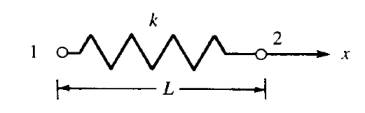
\includegraphics[width=15em]{phy_020_strs_06_03.jpg}

Sistemde bir yay görülüyor, bu yay üzerinde iki tane düğüm noktası seçtik,
onları takip edeceğiz, düğüm 1 ve 2. Düğümlerdeki yer değişimler $u_1,u_2$
olsun, yaydaki toplam değişim $\delta = u_1 - u_2$. Uygulanan kuvvet $T$
ise bir sabit $k$ üzerinden $T = k \delta$ eşitliği ortaya atılabilir.

Direngenlik matrisine gelirsek, sistemdeki tüm yer değişimleri şöyle gösterebiliriz,

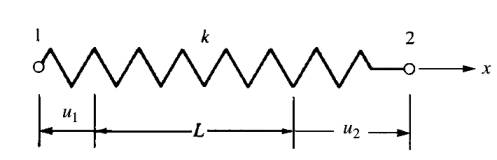
\includegraphics[width=15em]{phy_020_strs_06_04.jpg}

Sağ uçta yay $T$ kuvveti ile çekiliyorsa, bu durum sol uçta $-T$ tepkisel
kuvvete sebep olur. Ayrıca $u_1$'in sol yönü işaret ettiğine dikkat, çünkü yer
değişimin yönü pozitif yönün tersinde, yaydaki takip edilen nokta başlangıç
anının sol tarafında kalıyor, bu sebeple yön eksi.

$$
f_{1x} = -T, \quad f_{2x} = T
$$

Hepsini bir araya koyarsak

$$
T = -f_{1x} = k (u_2 - u_1)
$$

$$
T = f_{2x} = k (u_2 - u_1)
$$

Yani

$$
f_{1x} = k(u_1 - u_2)
$$

$$
f_{2x} = k(u_2 - u_1)
$$

Matris formunu kullanarak,

$$
\left[\begin{array}{ccc}
f_{1x} \\ f_{2x}
\end{array}\right] = 
\left[\begin{array}{ccc}
k & -k \\ -k & k
\end{array}\right]
\left[\begin{array}{ccc}
u_1 \\ u_2
\end{array}\right]
$$

İfadenin ortasındaki 2 x 2 matrisi direngenlik matrisidir.

Üstdüşüm (Superposition)

Eğer iki tane yay sistemini birbiriyle bağlı olarak işlemek istersek [4, sf. 38],
üstdüşüm tekniği kullanılabilir. Üstdüşüm basit bir matris toplamı ile
yapılabiliyor. Alttaki örneğe bakalım,

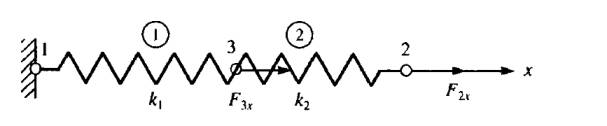
\includegraphics[width=20em]{phy_020_strs_06_02.jpg}

İki yay var, birbirlerine bağlılar, iki yayın sabitleri $k_1$, $k_2$
olsun. Her iki yayın direngenlik matrisi ayrı ayrı (tekabül eden yer değişim
değişkenleri matris kolon etiketi olarak gösteriliyor),

$$
k^{(1)} =
\begin{array}{cc} & \begin{array}{cc} u_1 & u_3 \end{array} \\ &
\left[
\begin{array}{cc}
k_1 & -k_1 \\ -k_1 & k_1
\end{array}
\right]
\end{array} 
\qquad
k^{(2)} =
\begin{array}{cc} & \begin{array}{cc} u_3 & u_2 \end{array} \\ &
\left[
\begin{array}{cc}
k_2 & -k_2 \\ -k_2 & k_2
\end{array}
\right]
\end{array}
$$

İki yay sistemini tek sistem haline getirmek aslında basit bir matris
toplamından ibaret fakat bu matrisin kolonları aynı değişkenlere tekabül ediyor
olmalı. O zaman her iki 2 x 2 matrisi genişletip 3 x 3 matrisi haline
getirirsek, değişken etiketlerini eşitlersek bu yeni iki matrisi
toplayabiliriz.

$$
k^{(1)} =
\begin{array}{cc} & \begin{array}{ccc} u_1 & u_2 & u_3 \end{array} \\ &
\left[
\begin{array}{ccc}
k_1 & 0 & -k_1 \\
0 & 0 & 0 \\
-k_1 & 0 & k_1
\end{array}
\right]
\end{array} \qquad
k^{(2)} =
\begin{array}{cc} & \begin{array}{ccc} u_1 & u_2 & u_3 \end{array} \\ &
\left[
\begin{array}{ccc}
0 & 0 & 0 \\
0 & k_2 & -k_2 \\
0 & -k_2 & k_2
\end{array}
\right]
\end{array} \qquad
$$

Dikkat edilirse mesela ilk matrisin $u_2$ kolonu tamamen sıfır çünkü 2 x 2
halindeki $k^{(1)}$ matrisinde bu değişken yoktu. Yeni genişletilmiş matrise
geçerken olmayan değişkenin kolonunu sıfırlarsak aslında aynı matrisi elde etmiş
oluruz.

Artık iki matrisi toplayabiliriz,

$$
\left[\begin{array}{ccc}
k_1 & 0 & -k_1 \\
0 & k_2 & -k_2 \\
-k_1 & -k_2 & k_1+k_2
\end{array}\right]
\left[\begin{array}{c}
u_1 \\ u_2 \\ u_3
\end{array}\right] =
\left[\begin{array}{c}
F_{1x} \\ F_{2x} \\ F_{3x}
\end{array}\right]
$$

Sınır Şartları (Boundary Conditions)

Resimde gösterilen örnekte sol tarafın duvara sabitlendiğini görüyoruz.
Sabitlenme demek notasyonumuz itibariyle $u_1 = 0$ demektir. Bu bir
sınır şartıdır, onu bir şekilde sistemimize dahil etmemiz gerekir.
Değeri üstteki sistemde yerine koyarsak,

$$
\left[\begin{array}{ccc}
k_1 & 0 & -k_1 \\
0 & k_2 & -k_2 \\
-k_1 & -k_2 & k_1+k_2
\end{array}\right]
\left[\begin{array}{c}
0 \\ u_2 \\ u_3
\end{array}\right] =
\left[\begin{array}{c}
F_{1x} \\ F_{2x} \\ F_{3x}
\end{array}\right]
$$

Matris sistemini cebirsel olarak tekrar açarsak,

$$
k_1(0) + (0) u_2 - k_1 u_3 = F_{1x}
$$

$$
0(0) + k_2 u_2 - k_2 u_3 = F_{2x}
$$

$$
-k_1 (0) - k_2 u_2 + (k_1+k_2) u_3 = F_{3x}
$$

elde edilir. Bu sistemde sadece ikinci ve üçüncü denklemi matris olarak
yazabiliriz,

$$
\left[\begin{array}{cc}
k_2 & -k_2 \\ -k_2 & k_1 + k_2 
\end{array}\right]
\left[\begin{array}{c}
u_1 \\ u_2
\end{array}\right] =
\left[\begin{array}{c}
F_{2x} \\ F_{3x}
\end{array}\right]
$$

Bu son matrisi elde etmek için bir anlamda önceki matrisin birinci satırı ve
kolonunu dışarı attık, kenara ayırdık, ve kalanlarla yeni bir sistem yarattık.
Fakat dikkat bu $F_{1x}$ sıfır demek değildir, onun hala bir ifadesi var,
$F_{1x} = -k_1 u_3$, ve bu eşitliği bir kez sistemin geri kalanının çözdükten
sonra dönüp ayrıca bulmamız gerekiyor.

Devam edelim, yeni sistemi çözersek,

$$
\left[\begin{array}{ccc}
u_2 \\ u_3
\end{array}\right] =
\left[\begin{array}{cc}
k_2 & -k_2 \\ -k_2 & k_1 + k_2 
\end{array}\right]^{-1}
\left[\begin{array}{c}
F_{2x} \\ F_{3x}
\end{array}\right]
$$

$$
= \left[\begin{array}{cc}
\dfrac{1}{k_2} + \dfrac{1}{k_1} & \dfrac{1}{k_1} \\
\dfrac{1}{k_1} & \dfrac{1}{k_1} 
\end{array}\right]
\left[\begin{array}{c}
F_{2x} \\ F_{3x}
\end{array}\right]
$$

$u_2,u_3$ bir kez elde edildikten sonra $F_{1x} = -k_1 u_3$ formülü
ile $F_{1x}$ elde edilebilir.

Gerinim Tensörü (Strain Tensor) 

Önce nesneleri nasıl temsil ettiğimizden bahsedelim [2]. Diyelim ki elimizde bir
patates var. Fakat bu patatesin matematiksel olarak bir anlamı yok. Eğer bu
nesneyi $R^3$ uzayında temsil etmek istiyorsak, onun üzerindeki belli seçilmiş
noktalar sayesinde bunu yapabiliriz.

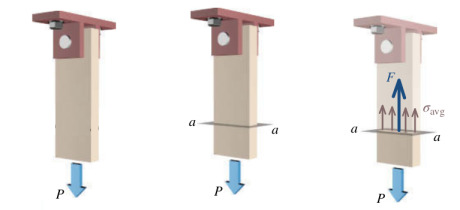
\includegraphics[width=8em]{phy_020_strs_01_01.jpg}

Nesne üzerindeki mavi noktalar bu seçilmiş noktaları gösteriyor.

Seçilmiş noktaların kordinatı bir referansa göre alınmalı, $e_1,e_2,e_3$
şeklinde bir baz bu işi yapabilir. Artık bu baza, kordinat sistemine izafi
olarak patates üzerindeki her noktayı bir vektör olarak temsil edebiliyoruz.
Altta örnek olarak üç tane seçilmiş noktayı gösterdik,

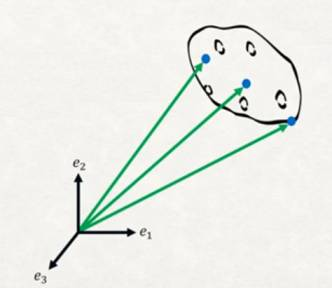
\includegraphics[width=13em]{phy_020_strs_01_02.jpg}

Daha fazla nokta da seçebilirdik, tüm seçilmiş noktalardan gelen vektörlerin
kümesi cisim hakkında bize bir konum, durum bilgisi verecektir, bu konuma biçim
değiştirme öncesi noktaların konumu $\Omega_0$ diyelim, ya da referans konumu.
Nesne üzerindeki değişimler, özellikle bu ders sonlu öğeler (finite elements
method, FEM) dersi olduğu için deformasyon değişimleri referans vektörlerinin
nasıl değiştiği üzerinden incelenebilir. İlk konumdaki bir vektörü, $X$ diyelim,
değişimi $f$ fonksiyonu yapıyor olsun, sonuç vektörü $x$ olacak, yani $x =
f(X)$.

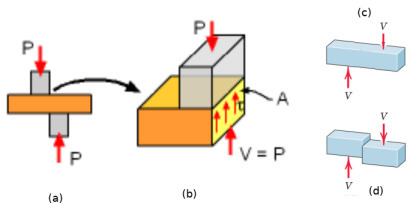
\includegraphics[width=17em]{phy_020_strs_01_03.jpg}

Üstteki resimde örnek bir değişim görüyoruz; yana kayma, dönme, uzama
var. Değişimi gerçekleştiren $f$ fonksiyonu. Bu ders için farz edilen $f$'nin
birebir ve örten (bijective) olduğu, liner cebirden hatırlarsak bu $f$'nin tersi
alınabilir olduğu anlamına geliyor, yani elimde deforme edilmiş konum var ise,
$f$'nin tersi ile başlangıç konumuna dönebilirim. Diğer bir faraziye fonksiyonun
sürekli (continuous), ve pürüzsüz (smooth), yani türevi alınabilir olduğu. Katı
cisim mekaniğinde türevi alınabilirlik önemli bir faraziyedir, gerçek hayatta
böyle mi, her zaman değil muhakkak, hatta bir bakıma bu sebepten dolayı FEM'e
ihtiyacımız var.

Ayrıca bize ileride lazım olabilecek bir üçüncü vektör $u$ da tanımlayabiliriz,
bu vektör varılan konumu referans konumuna direk ilintilendiriyor. Vektör $u$'ya
yer değişim fonksiyonu denir. Pozisyon fonksiyonu ile karıştırmayalım, o küçük
$x$, bu yer değişim fonksiyonu $u$.

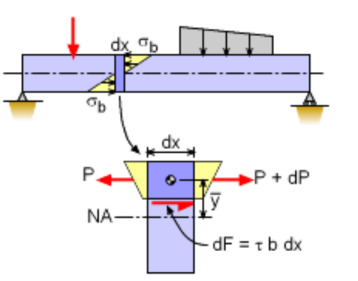
\includegraphics[width=17em]{phy_020_strs_01_05.jpg}

Fakat bu tüm grafiğe baktığımızda $u$'nun aslında vektör çıkartma operasyonunu
gösterdiğini fark edebiliriz, yani $u = x - X$.

Üç tür katı gövde değişimine bakalım şimdi, not katı demek gövde esneyip,
uzamıyor demek.

Katı Gövde Yer Değişimi: $x = X + c$, ki $c$ sabit bir vektör. Pür yer değişimi
olduğu için basit bir toplanma işlemi sadece. Şimdi bildiğimiz sonuç konumu
formülünü yazarsak, $u = x - X$ bu formülde önceki $x$'i geçirelim, $u = X + c -
X$ yani $u = c$.

Katı Gövde Dönüşü: $x = Q X$, formüldeki $Q$ bir dönüş matrisidir. Tekrar yer
değişim formülünü yazalım, $u = x - X$ ve önceki $x$'i yerine koyalım, $u = QX -
X$, tekrar düzenlersek, $u = (Q-I)X$.

Katı Gövde Hareketi: $x = QX + c$, bu kalem aslında önceki iki kalemin
birleşimi, hem dönüş hem de yer değişimi var. Çoğunlukla fizik problemlerinde bu
kavramdan bahsedilir. Yine $u$'yu düşünürsek $u = (Q-I)X + c$ elde ederiz.

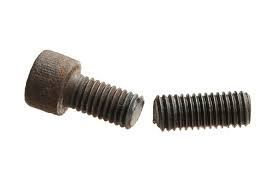
\includegraphics[width=10em]{phy_020_strs_01_04.jpg}

Bahsedilen değişim türleri üstte resmedildi, yanlız hala gerinim, esneme,
küçülme türü şekil değişimlerini görmedik. Diğerleri şunlar,

Her Yönde Uzama ve Küçülme (Uniform Extension and Contraction)

Her kordinat ekseninde uzama var ise, mesela $x_1 = k_1 X_1$, $x_2 = k_2 X_2$,
$x_3 = k_3 X_3$, ki $k_i > 0$ reel sayı olmak üzere. Bu değişimleri matris
ile şöyle gösterebiliriz,

$$
x = \left[\begin{array}{c}
x_1 \\ x_2 \\ x_3
\end{array}\right] =
\left[\begin{array}{ccc}
k_1 & 0   &   0 \\
0   & k_2 & 0 \\
0   & 0   & k_3
\end{array}\right]
\left[\begin{array}{c}
X_1 \\ X_2 \\ X_3 
\end{array}\right] =
\left[\begin{array}{c}
k_1 X_1 \\ k_2 X_2 \\ k_3 X_3 
\end{array}\right]
$$

Üstteki ifadeden pozisyon fonksiyonunu şöyle belirtebiliriz,

$$
u = x - X = \left[\begin{array}{ccc}
(k_1 - 1) X_1 \\ 
(k_2 - 1) X_2 \\ 
(k_3 - 1) X_3 
\end{array}\right]
$$

İki boyutta eğer hem $k_1$ hem $k_2$ 1'den büyükse her iki eksende esneme
görülürdü,

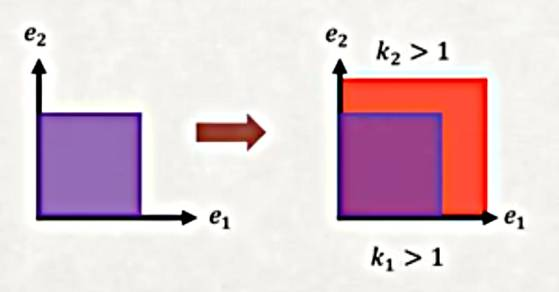
\includegraphics[width=10em]{phy_020_strs_01_06.jpg}

Eğer sadece $k_1 > 1$ ise o yönde büyüme olurdu, diğerinde değil. Eğer
$0 < k < 1$ ise küçülme, $k > 1$ ise büyüme, $k = 1$ değişim yok.

$k=0$ ya da $k<0$ fiziki dünyada mümkün değil, mesela $k<0$ durumunda nesnenin
tamamen kendi tersine dönmüş olması gerekiyor, bu da fiziksel olarak olamaz.

Basit Kaykılma (Simple Shear)

Üç boyutta $e_2$ etrafında bir kaykılma düşünüyor olsaydık, bunu

$$
x_1 = X_1 + k X_2, \qquad x_2 = X_2, \qquad x_3 = X_3
$$

ile temsil edebilirdik, $\theta$ açısında bir kaykılma için matris formunda

$$
x = \left[\begin{array}{ccc}
1 & \tan(\theta) & 0 \\
0 & 1 & 0 \\
0 & 0 & 1 
\end{array}\right]
\left[\begin{array}{c}
X_1 \\ X_2 \\ X_3
\end{array}\right] =
\left[\begin{array}{c}
X_1 + \tan(\theta) X_2 \\
X_2 \\
X_3
\end{array}\right] 
$$

$$
\implies u = x - X =
\left[\begin{array}{ccc}
\tan(\theta) X_2 \\
0 \\
0
\end{array}\right]
$$

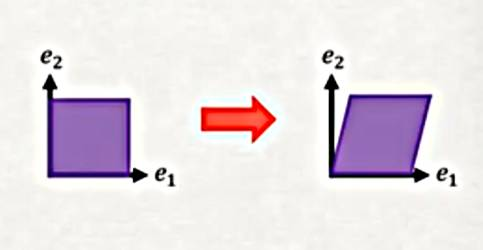
\includegraphics[width=10em]{phy_020_strs_01_07.jpg}

Pür Kaykılma (Pure Shear)

Bu tür şekil değiştirme birden fazla eksen bazında olabilir,

$$
x = \left[\begin{array}{ccc}
1               & \tan(\theta/2) & 0 \\
\tan(\theta/2) & 1              & 0 \\
0               & 0              & 1 
\end{array}\right]
\left[\begin{array}{c}
X_1 \\ X_2 \\ X_3
\end{array}\right] =
\left[\begin{array}{c}
X_1 + \tan(\theta/2) X_2 \\
\tan(\theta/2) X_1 + X_2  \\
X_3
\end{array}\right] 
$$

$$
\implies u = x - X =
\left[\begin{array}{ccc}
\tan(\theta / 2) X_2 \\
\tan(\theta / 2) X_1 \\
0
\end{array}\right]
$$

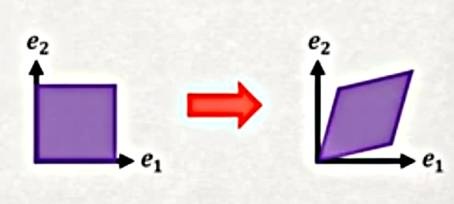
\includegraphics[width=10em]{phy_020_strs_01_08.jpg}

Nihayet gerinim konusunda geldik. Bu dersin en önemli konusu bu. Başta
gösterdiğimiz patatese dönelim, referans konumundaki bir mavi noktaya $X$'e
bakıyorduk, patatesi yamulttuğumuz zaman sonuç konumdaki $x$ elde ediliyordu,
her iki noktayı birbiriyle ilintilendiren aralarındaki $u$ vektörü idi.

Şimdi gerinim tensörünü türetmek için patateslere ikinci bir nokta
ekleyeceğiz. Referans konumda $X$ noktası ile bu ikinci nokta arasındaki vektör
$\ud X$ olacak, sonuç patatesindeki ikinci noktaya olan vektör $\ud x$.  Tabii
bu noktaları rasgele eklemedik, yamultan fonksiyon $\ud X$'i yamultunca $\ud x$
elde ettik, sonuç patatesteki ikinci noktaya böyle eriştik.

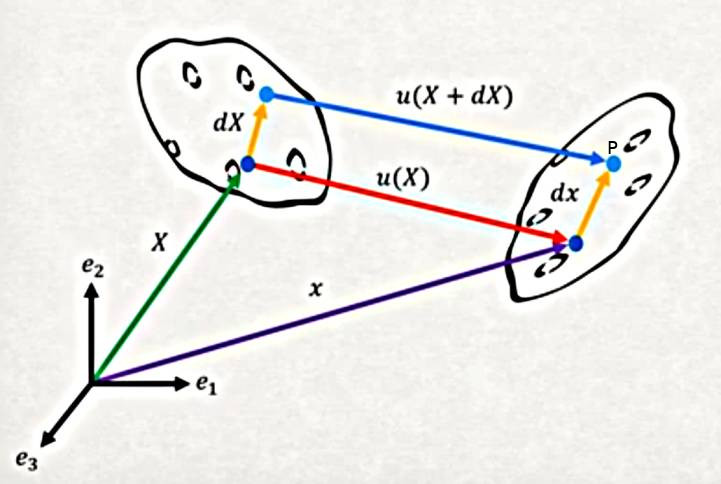
\includegraphics[width=15em]{phy_020_strs_01_09.jpg}

Şimdi diyelim ki orijinden ikinci patatesteki $P$ noktasına gitmek
istiyoruz. Bir yol $X$, $\ud X$, $u(X+\ud X)$ olabilirdi, bu vektörlerin toplamı
bizi $P$'ye götürür. Fakat daha kısa bir yol daha var, $x$, $\ud x$. Aynı
noktaya eriştiğimize göre bu iki yolun vektör toplamları birbirine eşit olmalı.
O zaman şu ifade doğrudur,

$$
x + \ud x = X + \ud X + u(X+\ud X)
$$

Eğer $x$'i sol taraftan sağa geçirirsem, ve biraz düzenleme sonrası,

$$
\ud x = \ud X + u(X+\ud X) - (x - X)
$$

Tabii daha önceden hatırlıyoruz ki $u(X) = (x - X)$ o zaman 

$$
\ud x = \ud X + u(X+\ud X) - u(X)
\mlabel{1}
$$

Üstteki ifade tanıdık bir kavrama dönüşmeye başladı, eşitliğin sağ tarafı kısmen
bir türeve, gradyana benzemiyor mu? Gradyan tanımı,

$$
\nabla u = \frac{u(X+\ud X) - u(X)}{\ud X}
$$

$\nabla u$'ya yer değişim gradyanı deniyor.  Bunu (1) ifadesine uydurmak için 

$$
\nabla u \ud X = u(X+\ud X) - u(X)
$$


Şimdi (1)'de yerine geçirelim,

$$
\ud x = \ud X + \nabla u \ud X
$$

Bir basitleştirme daha,

$$
\ud x = (I + \nabla u) \ud X
\mlabel{2}
$$

$I + \nabla u$ ifadesine şu şekilde erişmek mümkün, hatırlarsak
$x = X + u(X)$ idi. Eğer değişim gradyanı $F$ olarak $F = \partial x / \partial X$,
ya da $F_{ij} = \frac{\partial x_i}{\partial X_j}$ tanımlarsak [1, sf. 144], 

$$
\frac{\partial (X + u(X))}{\partial X} = 1  + \frac{\partial u}{\partial X} = F
$$

$$
F = I + \nabla u
$$

Üsttekini (2)'ye sokarsak,

$$
\ud x = F \ud X
$$

elde ederiz.

$F$'ye bakmanın bir diğer yolu $x = \Phi(X,t)$ tanımından hareketle doğal olarak
elde edilen

$$
\ud x = \frac{\partial x}{\partial X} \ud X
$$

formülü. Burada $F$ dediğimiz $\ud X$ sonsuz ufak büyüklüğü $\ud x$'e ceviren
şey, açılımı tabii ki $F = \partial x / \partial X$, ya da $F_{ij} = \frac{\partial x_i}{\partial X_j}$.
$x$ için farklı bir formül kullanınca mesela $x = X + u(x)$ bu durumda $F$
hesabı bizi $I + \nabla u$'ya götürecektir.

Devam edelim, dersin geri kalanında gerinim konusunu işlerken hep $\ud x = F \ud
X$ formülünü baz alacağız. Niye?  Çünkü gerinim bir uzunluk değişimidir ve
üstteki formül bana baştaki ufak fark vektörlerinin nasıl uzunluksal olarak
değişime uğradığını gösteriyor. Orijinal pozisyondaki değişim $\ud X$ biliniyor,
buradan değişim sonrasındaki $\ud x$'e geçerek o mesafeyi hesaplayabilirim.


Gradyanlar

Deformasyon ve yer değişim gradyanından bahsettik. Yer değişim gradyanı $\nabla
u$ bir tensör alan (field) sonucunu verir, çünkü $u$ bir vektör değerli
fonksiyondur. Yer değişim (displacement) gradyanı $\nabla u$'nun tam tanımı,

$$
\renewcommand*{\arraystretch}{2.5}
\nabla u = \frac{\partial u_i}{\partial X_j} =
\left[\begin{array}{ccc}
\dfrac{\partial u_1}{\partial X_1} & \dfrac{\partial u_1}{\partial X_2} & \dfrac{\partial u_1}{\partial X_3} \\
\dfrac{\partial u_2}{\partial X_1} & \dfrac{\partial u_2}{\partial X_2} & \dfrac{\partial u_2}{\partial X_3} \\
\dfrac{\partial u_3}{\partial X_1} & \dfrac{\partial u_3}{\partial X_2} & \dfrac{\partial u_3}{\partial X_3} 
\end{array}\right]
$$

Yamulma / Deformasyon Gradyanı $F$

$F$'nin formülü $F = I + \nabla u$ ise üstteki matristen hareketle bu basit
bir hesap,

$$
F = I + \nabla u = 
\left[\begin{array}{ccc}
1 & 0 & 0 \\ 0 & 1 & 0 \\ 0 & 0 & 1
\end{array}\right] + 
\renewcommand*{\arraystretch}{2.5}
\left[\begin{array}{ccc}
\dfrac{\partial u_1}{\partial X_1} & \dfrac{\partial u_1}{\partial X_2} & \dfrac{\partial u_1}{\partial X_3} \\
\dfrac{\partial u_2}{\partial X_1} & \dfrac{\partial u_2}{\partial X_2} & \dfrac{\partial u_2}{\partial X_3} \\
\dfrac{\partial u_3}{\partial X_1} & \dfrac{\partial u_3}{\partial X_2} & \dfrac{\partial u_3}{\partial X_3} 
\end{array}\right]
$$

Üstteki toplam aslında alttaki kısmi türev matrisine eşittir,

$$
\renewcommand*{\arraystretch}{2.5}
F = \left[\begin{array}{ccc}
\dfrac{\partial x_1}{\partial X_1} & \dfrac{\partial x_1}{\partial X_2} & \dfrac{\partial x_1}{\partial X_3} \\
\dfrac{\partial x_2}{\partial X_1} & \dfrac{\partial x_2}{\partial X_2} & \dfrac{\partial x_2}{\partial X_3} \\
\dfrac{\partial x_3}{\partial X_1} & \dfrac{\partial x_3}{\partial X_2} & \dfrac{\partial x_3}{\partial X_3} 
\end{array}\right] =
\frac{\partial x_i}{\partial X_j}
$$

Yani elde ettiğimiz pozisyon fonksiyonunun gradyanıdır. Nihai olarak eşitliği
$\nabla u = F - I$ olarak ta gösterebilirdik, yani,

$$
\renewcommand*{\arraystretch}{2.5}
\nabla u =
\left[\begin{array}{ccc}
\dfrac{\partial u_1}{\partial X_1} & \dfrac{\partial u_1}{\partial X_2} & \dfrac{\partial u_1}{\partial X_3} \\
\dfrac{\partial u_2}{\partial X_1} & \dfrac{\partial u_2}{\partial X_2} & \dfrac{\partial u_2}{\partial X_3} \\
\dfrac{\partial u_3}{\partial X_1} & \dfrac{\partial u_3}{\partial X_2} & \dfrac{\partial u_3}{\partial X_3} 
\end{array}\right] = 
\left[\begin{array}{ccc}
\dfrac{\partial x_1}{\partial X_1} & \dfrac{\partial x_1}{\partial X_2} & \dfrac{\partial x_1}{\partial X_3} \\
\dfrac{\partial x_2}{\partial X_1} & \dfrac{\partial x_2}{\partial X_2} & \dfrac{\partial x_2}{\partial X_3} \\
\dfrac{\partial x_3}{\partial X_1} & \dfrac{\partial x_3}{\partial X_2} & \dfrac{\partial x_3}{\partial X_3} 
\end{array}\right] -
\renewcommand*{\arraystretch}{1.0}
\left[\begin{array}{ccc}
1 & 0 & 0 \\ 0 & 1 & 0 \\ 0 & 0 & 1
\end{array}\right]
$$





Şimdi Lagrange (Green) tensörüne gelelim.

Gerinim, yamulma sonucu uzunluk değişimidir. $\ud x = F \ud X$ formülü vektörler
arası değişimi gösteriyor, formülü vektör uzunluğu (norm) kullanacak şekilde
değişterebiliriz. Eşitliğin iki tarafını kendisi ile noktasal çarpıma tabi
tutarım, böylece her iki tarafta norm elde ederim,

$$
\ud x \cdot \ud x  = (F \ud X) \cdot (F \ud X)
$$

$$
||\ud x||^2  = \ud X \cdot (F^T F) \ud X
$$

Son eşitlik ortaya çıktı çünkü bir $Ax$ örneği üzerinden bakarsak,

$$
Ax \cdot Ax = (Ax)^T Ax = x^T A^T (Ax) = x^T (A^T A) x  = x \cdot (A^T A) x
$$

Ana konumuza dönersek, iki üstteki $F^T F$ grubuna $C$ diyelim, bu büyüklük
Sağ Cauchy-Green Yamulma Tensörü (Right Cauchy-Green Deformation Tensor)
olarak biliniyor.

Bir zihin egzersizi yapalım, eğer $C = F^T F = I$ yani $C$ birim matristir
dersem ne olur? O zaman

$$
||\ud x||^2  = \ud X \cdot I \ud X = \ud X \cdot \ud X
$$

$$
||\ud x||^2 = ||\ud X||^2
$$

Bu bize uzunlukları değişmediği bir ortamı gösteriyor, demek ki elimizde bir
katı-gövde hareketi (rigid-body motion) bulunuyor. Gövdede hiç esneme, gerinim,
uzama yok, obje şeklen olduğu gibi kalıyor.

Normal şartlarda $F = (I+\nabla u)$ ve $F^T F$ birim matris değil, bu durumda
tüm $C$'yi açarsak,

$$
C = F^T F = (I+\nabla u)^T (I+\nabla u) =
I + \nabla u + \nabla u^T + \nabla u^T \nabla u
$$

Katı-gövde için $C = I$ demiştik, üstteki son ifadede $C = I + ...$  gibi
bir açılım var, nokta nokta olan yerler tabii ki diğer semboller. Ama
tekrar katı-gövde durumunu düşünürsek, o durumda $C = I$ olacağı için
üstteki formülde $I$ sonrası gelen,

$$
.. + \nabla u + \nabla u^T + \nabla u^T \nabla u
$$

terimleri tamamen sıfır demektir.

Şimdi Cauchy-Green tensörünü tekrar tanımlayalım,

$$
C = I + 2 \epsilon_{Green} 
$$

öyle ki 

$$
\epsilon_{Green} = \frac{1}{2} (\nabla u + \nabla u^T + \nabla u^T \nabla u )
\mlabel{3}
$$

Not: $C$ içinde 2 ile çarpım var $\epsilon_{Green}$ içinde 1/2 bunlar birbirini
iptal eder ama 1/2 kullanımı karesel formlarda yaygın şekilde kullanılır,
basitleştirici bir amacı var muhakkak. 

Böylece Green Gerinim Tensörünü tanımlamış olduk.

Tensörün bizim için faydalı bazı özellikleri var.

1) Simetrik: Bu özellik hesapları rahatlaştırır, özellikle yaklaşık
hesaplara gelince simetrinin faydalarını göreceğiz. 

2) Sonlu (finite) yamulmalar için geçerli: Tensör hesabı için $\nabla u$
kullanılır, onun için de yer değişim fonksiyonu yeterlidir. Bunlar varsa geçerli
bir formül eldedir.

Sonsuz Küçük Gerinim Tensörü (Infinitesimal Strain Tensor)

Green gerinim tensörünü gördük, kuvvetli bir yaklaşım ama bizim daha çok
kullanacağımız şimdi anlatacağımız. Niye? Çünkü Green tensörü sonlu
deformasyonlar / yamulmalar için geçerli ama çoğu uygulamada bize lazım olan çok
ufak yamulmalar. Ufak derken, önceki dersteki (3) formülünden hareketle, oradaki
en son terimi hatırlarsak, çok ufak yamulmalar için $\nabla u^T \nabla u << \nabla u$ 
olur, yani ufak değişimlerde o karesel işlem $\nabla u$'dan daha ufak sonuç
verir. O zaman belli durumlarda son terim yaklaşık sıfır kabul edilebilir,
$\nabla u^T \nabla u \approx 0$. Green tensörü bu durumlarda yaklaşık
olarak alttaki gibi olur,

$$
\epsilon_{Green} \approx \frac{1}{2} (\nabla u + \nabla u^T )
$$

Tüm öğeleri gözükecek şekilde [3, 4.3.2.2], 

$$
\left[\begin{array}{ccc}
  \frac{\partial u_1}{\partial X_1} &
  \frac{1}{2}(\frac{\partial u_1}{\partial X_2} + \frac{\partial u_2}{\partial X_1} ) & 
  \frac{1}{2}(\frac{\partial u_1}{\partial X_3} + \frac{\partial u_3}{\partial  X_1} )
\\
  \frac{1}{2}(\frac{\partial u_1}{\partial X_2} + \frac{\partial u_2}{\partial X_1} ) &
  \frac{\partial u_2}{\partial X_2} &
  \frac{1}{2}(\frac{\partial u_2}{\partial X_3} + \frac{\partial u_3}{\partial X_2} )
\\
  \frac{1}{2}(\frac{\partial u_1}{\partial X_3} + \frac{\partial u_3}{\partial X_1} ) &
  \frac{1}{2}(\frac{\partial u_2}{\partial X_3} + \frac{\partial u_3}{\partial X_2} ) &
  \frac{\partial u_3}{\partial X_3} 
\end{array}\right]
$$

Bileşen formunda

$$
\epsilon_{ij} = \frac{1}{2}\left(
\frac{\partial u_i}{\partial X_j} + \frac{\partial u_j}{\partial X_i}
\right)
$$

Bu tensör de simetrik, fakat sadece ufak şekil değişimleri, yamulmalar için
geçerli. Fakat zaten, mesela inşaat mühendisliği durumunda, binalar, demir
kirişler (beam) ile iş yaptığımız zaman, bu tür şekil değişimi faraziyesi
yeterli. Çünkü eh, biraz düşünürsek eğer binamız büyük şekil değişimleri
yaşıyorsa önümüzde daha büyük bir problem var demektir.

Kaynaklar

[1] Kim, {\em Introduction to Non-linear Finite Element Analysis}

[2] Petitt, {\em Intro to the Finite Element Method}, University of Alberta,
    \url{https://www.youtube.com/watch?v=2iUnfPRk6Ro&list=PLLSzlda_AXa3yQEJAb5JcmsVDy9i9K_fi}
    
[3] Adeeb, {\em Introduction to Solid Mechanics, Online Book},
    \url{https://engcourses-uofa.ca/books/introduction-to-solid-mechanics/}

[4] Logan, {\em A First Course in the Finite Element Method}

[5] Bayramlı, {\em Hesapsal Bilim, Ders 1-8}

    
\end{document}



